\documentclass[14pt]{extreport}
\usepackage{gost}
\usepackage{lscape}
\usepackage{lscape}
\usepackage[justification=centering]{caption}
\usepackage{diagbox}
\usepackage{graphics}
%Тут можно вставить дополнительные пакеты

\setstretch{1.5}

\begin{document}
\pagestyle{empty} %  выключаем нумерацию
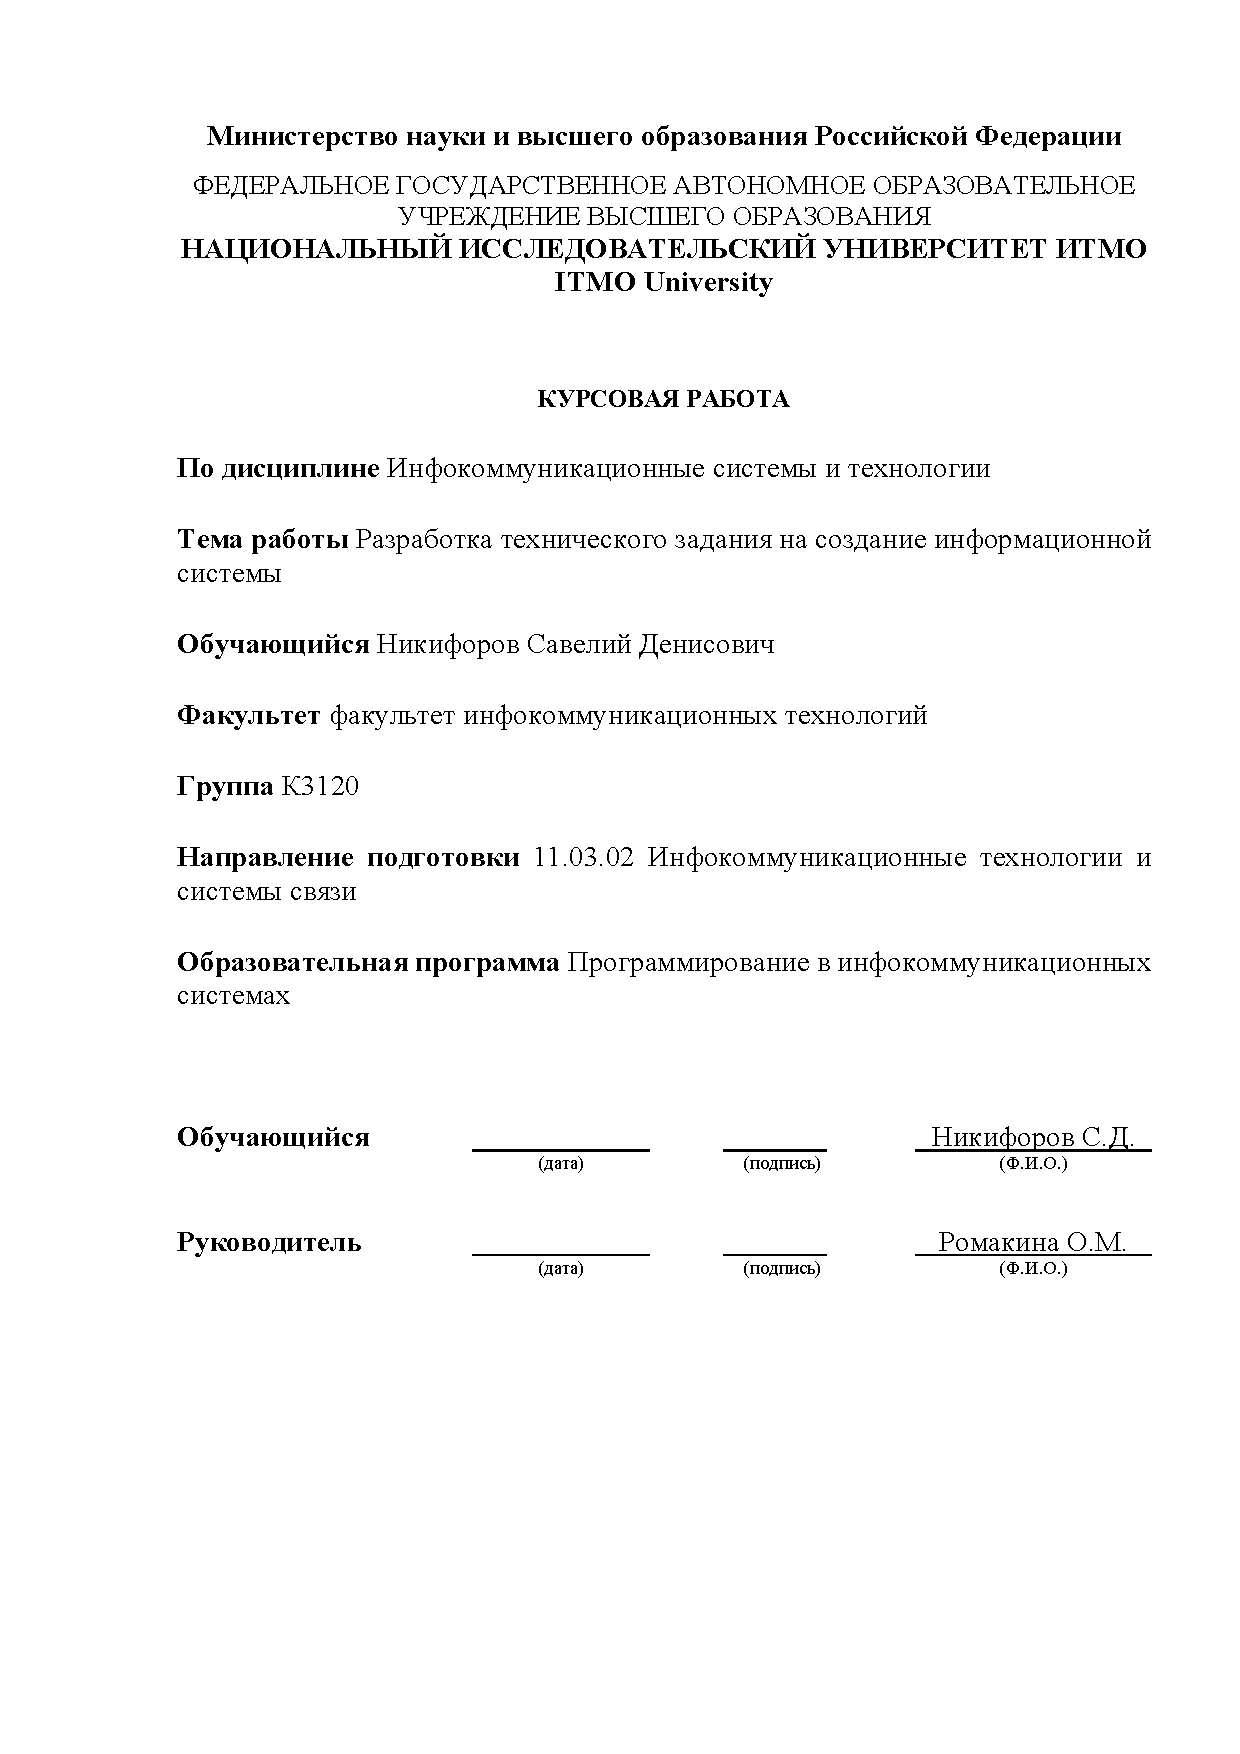
\includepdf[pages=-,pagecommand={}]{titulCourse.pdf}

\pagestyle{plain} % включаем нумерацию

\chapter{Создание углубленного сценария использования базы данных.}

В данном разделе будет представлен углубленный сценарий использования базы данных магазина по продаже овощей и фруктов.


Магазин овощей и фруктов предоставляет возможность продажи как в розницу так и в формате интернет-магазина. У магазина два варианта покупателей: Анонимный пользователь и зарегистрированный в системе. Анонимным пользователем является человек, который произвел покупку без авторизации в системе. Например: если покупка была произведена в физическом магазине без использования программы лояльности, или же без авторизации в онлайн-магазине. Внутри системы существует роль продавца-консультанта, который может вносить данные о заказах, которые оформляет пользователь. Если заказ был произведен онлайн, то данные о заказе вносится автоматизированной системой. Дальнейшее сопровождение заказа выполняется при помощи продавцов-консультантов. В штате компании существует складской работник, который взаимодействует с товарами на складе. Он оперирует с занесением полученным от поставщиков продуктов, также следит за сроками годности позиций на складе (существует отдельное предоставление). Для автоматизированной системы существует представление (view) которое возвращает вычисленные данные (оставшийся срок годности от партии, базовая стоимость, стоимость со скидкой) для отображения на клиенте онлайн-магазина.

\chapter{Определение ключевых объектов системы}

    \section{Потенциальные объекты системы}
        В процессе анализирования предметной области были выделены следующие примерные бизнес-сущности, которые должны быть отображены в базе данных.

        \begin{itemize}
            \item Покупатель
            \item Работники
            \item Продажа
            \item Позиция продажи
            \item Доставка
            \item Товар на складе
            \item Поставка
            \item Подрядчик
        \end{itemize}
    
    \section{Примерный состав интервью с работником организации}

        \begin{enumerate}
            \item Возможные товары:
            
            \begin{itemize}
                \item Вопрос: Какие основные категории овощей фруктов у вас продаются?
                \item Ответ: У нас в магазине продаются свежие овощи различных видов, включая корнеплоды, листовые овощи, и бобовые. А также цитрусовые, субтропические и тропические фрукты.
            \end{itemize}
            
            \item Процессы закупки и продажи:
            
            \begin{itemize}
                \item Вопрос: Как происходит закупка овощей для магазина?
                \item Ответ: Мы сотрудничаем с несколькими поставщиками, которые поставляют свежие овощи ежедневно. Закупка осуществляется на основе спроса и сезонности.
            \end{itemize}

            \item Клиентская информация:
            
            \begin{itemize}
                \item Вопрос: Какую информацию о клиентах вы собираете?
                \item Ответ: Мы сохраняем базовую информацию о клиентах, такую как их имена, контактные данные и адреса доставки.
            \end{itemize}

            \item{Операционные потребности:}
            \begin{itemize}
                \item Вопрос: Какие операционные задачи вызывают больше всего трудностей в повседневной работе?
                \item Ответ: Один из основных вызовов - это система снятия продукта с продажи из-за истечения срока хранения. Кроме того, иногда у нас бывают проблемы с хранениям адресов доставки.
            \end{itemize}

            \item{Сценарий использования базы данных:}
            \begin{itemize}
                \item Вопрос: Какие основные функции вы ожидаете от базы данных?
                \item Ответ: Мы бы хотели, чтобы база данных помогала нам в учете овощей, управлении ими, формировании заказов и предоставлении отчетов о продажах.
            \end{itemize}

            \item{Потенциальные атрибуты и требования:}
            \begin{itemize}
                \item Вопрос: Какие данные вы считаете важными для учета овощей?
                \item Ответ: Важными данными будут дата поступления товара, срок годности, количество на складе и информация о поставщиках.
            \end{itemize}

            \item{Системы, с которыми может взаимодействовать база данных:}
            \begin{itemize}
                \item Вопрос: Используете ли вы уже какие-то программные решения для управления магазином?
                \item Ответ: На данный момент у нас нет автоматизированных систем. Но мы готовы к внедрению новой базы данных, которая может интегрироваться с кассовой системой.
            \end{itemize}
        \end{enumerate}
    
    \section{Определение атрибутов и первичных ключей}

    \subsection*{Сущность <<Пользователь системы>>}

            \begin{table}[H]
                \begin{tabular}{|p{0.2\linewidth}|p{0.3\linewidth}|p{0.2\linewidth}|p{0.2\linewidth}|}
                    \hline
                    Наименование атрибута & Обязательный/не обязательный (*/o) & уникальный идентификатор (\#) & Тип для логической модели
                    \\ \hline
                    Id & * & \# & Числовой \\ \hline
                    FirstName & o & & Символьный\\ \hline
                    SecondName & o & & Символьный\\ \hline
                    LastName & o & & Символьный \\ \hline
                    Email & * & (\#) & Символьный  \\ \hline
                    PhoneNumber & о & & Символьный\\ \hline
                    Type & * & & Числовой \\ \hline
                \end{tabular}

                \caption{Описание сущности <<Пользователь>>.}
            \end{table}
        
        Сущность пользователь предоставляет всех пользователей системы,%
         которые могут взаимодействовать с системой. Атрибут <<Type>> %
          определяется принадлежность пользователя к системе акций.

    \subsection*{Сущность <<Продажа>>}

        \begin{table}[H]
            \begin{tabular}{|p{0.2\linewidth}|p{0.3\linewidth}|p{0.2\linewidth}|p{0.2\linewidth}|}
                \hline
                Наименование атрибута & Обязательный/не обязательный (*/o) & уникальный идентификатор (\#) & Тип для логической модели
                \\ \hline
                Id & * & \# & Числовой \\ \hline
                User & о & & Числовой\\ \hline
                Manager & * & & Числовой\\ \hline
                Shipping & o & & Числовой \\ \hline
                Discount & o & & Денежный \\ \hline  
                FinalPrice & * & & Денежный \\ \hline
                Status & * & & Строковый \\ \hline
            \end{tabular}
            \caption{Описание сущности <<Продажа>>.}
        \end{table}

        Сущность <<Продажа>> отображает процесс покупки какого-либо товара. Атрибут <<Status>> предполагает записи справочной таблицы о возможных состояниях заказа.
    
        \subsection*{Сущность <<Продажа>>}

        \begin{table}[H]
            \begin{tabular}{|p{0.2\linewidth}|p{0.3\linewidth}|p{0.2\linewidth}|p{0.2\linewidth}|}
                \hline
                Наименование атрибута & Обязательный/не обязательный (*/o) & уникальный идентификатор (\#) & Тип для логической модели
                \\ \hline
                Id & * & \# & Числовой \\ \hline
                User & о & & Числовой\\ \hline
                Manager & * & & Числовой\\ \hline
                Shipping & o & & Числовой \\ \hline
                Discount & o & & Денежный \\ \hline  
                FinalPrice & * & & Денежный \\ \hline
                Status & * & & Строковый \\ \hline
            \end{tabular}
            \caption{Описание сущности <<Продажа>>.}
        \end{table}

        Сущность <<Продажа>> отображает процесс покупки какого-либо товара. Атрибут <<Status>> предполагает записи справочной таблицы о возможных состояниях заказа.
    
    \subsection*{Сущность <<Позиция продажи>>}

        \begin{table}[H]
            \begin{tabular}{|p{0.2\linewidth}|p{0.3\linewidth}|p{0.2\linewidth}|p{0.2\linewidth}|}
                \hline
                Наименование атрибута & Обязательный/не обязательный (*/o) & уникальный идентификатор (\#) & Тип для логической модели
                \\ \hline
                Sell & * & \# & Числовой\\ \hline
                Item & * & \# & Числовой \\ \hline
                Amount & * & & Числовой \\ \hline
            \end{tabular}
            \caption{Описание сущности <<Позиция продажи>>.}
        \end{table}

        Сущность <<Позиция продажи>> является сущностью пересечения.


    \subsection*{Сущность <<Товар на складе>>}

        \begin{table}[H]
            \begin{tabular}{|p{0.2\linewidth}|p{0.3\linewidth}|p{0.2\linewidth}|p{0.2\linewidth}|}
                \hline
                Наименование атрибута & Обязательный/не обязательный (*/o) & уникальный идентификатор (\#) & Тип для логической модели
                \\ \hline
                Id & * & \# & Числовой \\ \hline
                Shipment & * & & Числовой\\ \hline
                RealizationDate & o & & Дата и время \\ \hline
                Name & * &  & Символьный  \\ \hline
                BaseCostByUnit & * & & Денежный \\ \hline
                Amount & * & & Денежный \\ \hline 
            \end{tabular}
            \caption{Описание сущности <<Товар на складе>>.}
        \end{table}

        Атрибут поставка предоставляет определенную поставку, которая прибыла в магазин по документам.
    
    \subsection*{Сущность <<Доставка>>}

        \begin{table}[H]
            \begin{tabular}{|p{0.2\linewidth}|p{0.3\linewidth}|p{0.2\linewidth}|p{0.2\linewidth}|}
                \hline
                Наименование атрибута & Обязательный/не обязательный (*/o) & уникальный идентификатор (\#) & Тип для логической модели
                \\ \hline
                Id & * & \# & \\ \hline
                Adress & * & & Символьный\\ \hline
                DeliveryTime & o & & Дата и время \\ \hline
                Contractor & * & & Целочисленный \\ \hline
            \end{tabular}
            \caption{Описание сущности <<Доставка>>.}
        \end{table}

        Атрибут <<Id>> является искуственным первичным ключем, для однозначного опредления доставки в системе.
    
    \subsection*{Сущность <<Поставка>>}

        \begin{table}[H]
            \begin{tabular}{|p{0.25\linewidth}|p{0.3\linewidth}|p{0.2\linewidth}|p{0.2\linewidth}|}
                \hline
                Наименование атрибута & Обязательный/не обязательный (*/o) & уникальный идентификатор (\#) & Тип для логической модели
                \\ \hline
                Id & * & \# & \\ \hline
                DocumentNumber & * & (\#) & Символьный\\ \hline
                Date & * & & Дата и время \\ \hline
                Provider & * & & Символьный \\ \hline
                Contactor & * & & Числовой \\ \hline
            \end{tabular}
            \caption{Описание сущности <<Поставка>>.}
        \end{table}

    \subsection*{Сущность <<Подрядчики>>}

        \begin{table}[H]
            \begin{tabular}{|p{0.25\linewidth}|p{0.3\linewidth}|p{0.2\linewidth}|p{0.2\linewidth}|}
                \hline
                Наименование атрибута & Обязательный/не обязательный (*/o) & уникальный идентификатор (\#) & Тип для логической модели
                \\ \hline
                INN & * & \# & \\ \hline
                ContactNumber & * &  & Символьный\\ \hline
                CompanyName & * & (\#) & Дата и время \\ \hline
                Description & о & & Символьный \\ \hline
            \end{tabular}
            \caption{Описание сущности <<Подрядчик>>.}
        \end{table}
    
    \section{Определение бизнесс правил}

    Для данной системы характерны следующие бизнес-правила:
    \begin{itemize}
        \item Покупатель может забрать заказ как лично, так и заказать доставку
        \item Сведения о покупках хранятся в базе данных ввиде заказов
        \item Покупатели приобретают товары, располагающиеся на складе
        \item Покупатель может получить скидку, если зарегестрирован в системе с заполнением ФИО
        \item Доставка осуществляется подрядной организацией
        \item Товары, по истечению срока реализации требуется списать
        \item Поставки продуктов реализует стороний подрядчик
    \end{itemize}
    
    \begin{landscape}
        
    
    \section{Матрица связей}
    
    

    \begin{table}[H]
        \begin{tabular}{|p{0.13\linewidth}|p{0.13\linewidth}|p{0.13\linewidth}|p{0.13\linewidth}|p{0.13\linewidth}|p{0.13\linewidth}|p{0.13\linewidth}|}
            \hline
            \diagbox[width=7.55em]& User & Sell & Item & Delivery & ItemOnStock & Suply
            \\ \hline
            
            User & \diagbox[width=7.55em] & & & & & \\ \hline 

            Sell & Triggered by  & \diagbox[width=7.55em] & & & & \\ \hline

            Item & & & \diagbox[width=7.55em] & & & \\ \hline
            
            Delivery & & & & \diagbox[width=7.55em] & & \\ \hline

            ItemOnStock & & & & & \diagbox[width=7.55em] & \\ \hline

            Suply & & & & & & \diagbox[width=7em] \\ \hline

        \end{tabular}
    \end{table}
    \end{landscape}

\end{document} 